
\documentclass[border=10pt]{standalone}
\usepackage{pgfplots}
\pgfplotsset{compat=1.18}
\begin{document}
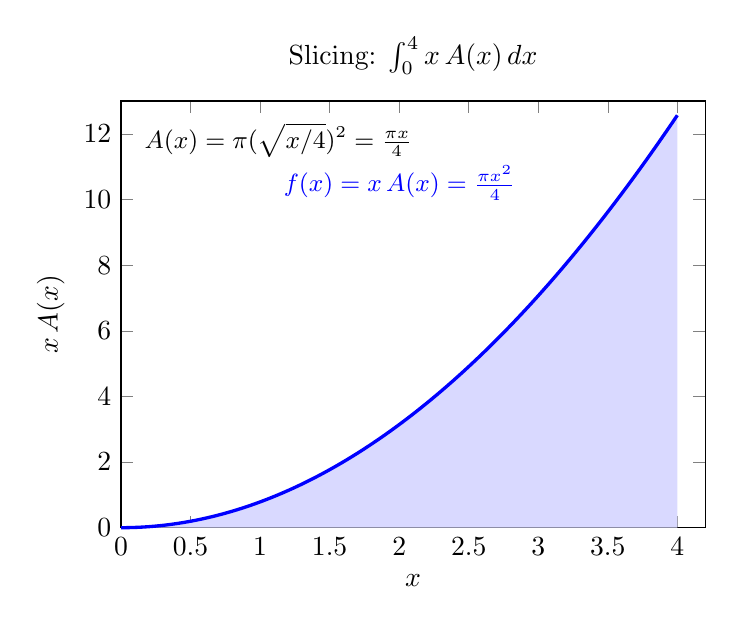
\begin{tikzpicture}
\begin{axis}[
    xlabel=$x$, ylabel=$x\,A(x)$,
    xmin=0, xmax=4.2,
    ymin=0, ymax=13,
    width=9cm, height=7cm,
    title={Slicing: $\int_0^4 x\,A(x)\,dx$},
    clip=false,
]
\addplot[fill=blue!15, draw=none, domain=0:4, samples=100] {pi*x^2/4} \closedcycle;
\addplot[blue, very thick, domain=0:4, samples=100] {pi*x^2/4};
\node[blue, font=\small, anchor=west] at (axis cs:1.1,10.5) {$f(x)=x\,A(x)=\frac{\pi x^2}{4}$};
\node[font=\small, anchor=west] at (axis cs:0.1,11.8) {$A(x)=\pi(\sqrt{x/4})^2=\frac{\pi x}{4}$};
\end{axis}
\end{tikzpicture}
\end{document}
